

\section{Rights and Privileges}

\subsection{Extended Rights}
\begin{itemize}
    \item \href{https://learn.microsoft.com/en-us/windows/win32/adschema/extended-rights}{Extended Rights}
\end{itemize}
\subsection{Built-in AD Groups}

AD contains many default or built-in security groups, some of which grant their
members powerful rights and privileges which can be abused to escalate
privileges within a domain and ultimately gain Domain Admin or \verb+SYSTEM+ privileges on a Domain Controller. Membership in many of these groups should be tightly managed as excessive group membership/privileges is a common flaw in many AD networks that attackers look to abuse. Some of the most common built-in groups are listed below.


\begin{xltabular}{\linewidth}{|l|X|}
    \hline
Group Name &	Description \\
    \hline
Account Operators &	can create and modify most types of accounts,
including those of users, local groups, and global groups, and members can log
in locally to domain controllers. They cannot manage the Administrator account,
administrative user accounts, or members of the Administrators, Server
Operators, Account Operators, Backup Operators, or Print Operators groups. \\
Administrators &	Members have full and unrestricted access to a computer or an
entire domain if they are in this group on a Domain Controller.\\
    \hline
Backup Operators &	can back up and restore all files on a computer,
regardless of the permissions set on the files. Backup Operators can also log
on to and shut down the computer. Members can log onto DCs locally and should
be considered Domain Admins. They can make shadow copies of the
SAM/ \gls{win:NTDS.DIT} database, which, if taken, can be used to extract credentials and other juicy
info.\\
    \hline
DnsAdmins &	have access to network DNS information. The group will only
be created if the DNS server role is or was at one time installed on a domain
controller in the domain.\\
    \hline
Domain Admins &	Members have full access to administer the domain and are
members of the local administrator's group on all domain-joined machines.\\
    \hline
Domain Computers &	Any computers created in the domain (aside from domain
controllers) are added to this group.\\
    \hline
Domain Controllers &	Contains all DCs within a domain. New DCs are added to this
group automatically.\\
    \hline
Domain Guests &	This group includes the domain's built-in Guest account.
Members of this group have a domain profile created when signing onto a
domain-joined computer as a local guest.\\
    \hline
Domain Users &	This group contains all user accounts in a domain. A new user
account created in the domain is automatically added to this group.\\
    \hline
Enterprise Admins &	Membership in this group provides complete configuration
access within the domain. The group only exists in the root domain of an AD
forest. Members in this group are granted the ability to make forest-wide
changes such as adding a child domain or creating a trust. The Administrator
account for the forest root domain is the only member of this group by
default.\\
    \hline
Event Log Readers &	Members can read event logs on local computers. The group
is only created when a host is promoted to a domain controller.\\
    \hline
Group Policy Creator Owners &	Members create, edit, or delete Group Policy
Objects in the domain.\\
    \hline
Hyper-V Administrators &	Members have complete and unrestricted access to all
the features in Hyper-V. If there are virtual DCs in the domain, any
virtualization admins, such as members of Hyper-V Administrators, should be
considered Domain Admins.\\
    \hline
IIS\_IUSRS &	This is a built-in group used by Internet Information Services
(IIS), beginning with IIS 7.0.\\
    \hline
Pre–Windows 2000 Compatible Access &	This group exists for backward
compatibility for computers running Windows NT 4.0 and earlier. Membership in
this group is often a leftover legacy configuration. It can lead to flaws where
anyone on the network can read information from AD without requiring a valid AD
username and password.\\
    \hline
Print Operators &	Members can manage, create, share, and delete printers that
are connected to domain controllers in the domain along with any printer
objects in AD. Members are allowed to log on to DCs locally and may be used to
load a malicious printer driver and escalate privileges within the domain.\\
    \hline
Protected Users &	Members of this group are provided additional protections
against credential theft and tactics such as Kerberos abuse.\\
    \hline
Read-only Domain Controllers &	Contains all Read-only domain controllers in
the domain.\\
    \hline
Remote Desktop Users &	This group is used to grant users and groups permission
to connect to a host via Remote Desktop (RDP). This group cannot be renamed,
deleted, or moved.\\
    \hline
Remote Management Users &	This group can be used to grant users remote access
to computers via Windows Remote Management (WinRM)\\
    \hline
    Schema Admins &	Members can modify the \gls{win:schema}, which is the
way all objects with AD are defined. This group only exists in the root domain
of an AD forest. The Administrator account for the forest root domain is the
only member of this group by default.\\
    \hline
Server Operators &	This group only exists on domain controllers. Members can
modify services, access SMB shares, and backup files on domain controllers. By
default, this group has no members.\\
    \hline
\end{xltabular}

\subsection{User Rights Assignment}

Depending on their current group membership, and other factors such as
privileges that administrators can assign via Group Policy (GPO), users can
have various rights assigned to their account. 

This Microsoft article on User Rights Assignment provides a detailed explanation of each of the user rights that can be set in Windows. 
\url{https://docs.microsoft.com/en-us/windows/security/threat-protection/security-policy-settings/user-rights-assignment}

some rights granted to an account can lead to unintended consequences such as privilege escalation 
or access to sensitive files. 

For example, write access over a Group Policy Object (GPO) applied to an OU
containing one or more users controled we could potentially leverage a tool
such as SharpGPOAbuse (\url{https://github.com/FSecureLABS/SharpGPOAbuse}) to assign targeted rights to a user. 
We may perform many actions in the domain to further our access with these new
rights. A few examples include :

\begin{tabularx}{\linewidth}{|l|X|}
    \hline
Privilege i&	Description \\
    \hline
SeRemoteInteractiveLogonRight &	could give our target user the
right to log onto a host via Remote Desktop (RDP). \\
    \hline
SeBackupPrivilege &	grants the ability to create system backups (copies of
    sensitive system files \verb+SAM+, \verb+SYSTEM Registry hives+ and
\gls{win:NTDS.DIT})\\ 
    \hline
SeDebugPrivilege &	allows  to debug and adjust the memory of a
process (Mimikatz to read the memory space of the LSASS process).\\
    \hline
SeImpersonatePrivilege & allows to impersonate a token of
a privileged account such as \verb+NT AUTHORITY\SYSTEM+. This could be leveraged with
a tool such as JuicyPotato, RogueWinRM, PrintSpoofer, etc., to escalate
privileges on a target system.\\
    \hline
SeLoadDriverPrivilege &	load and unload device
drivers that could potentially be used to escalate privileges or compromise a
system.\\
    \hline
SeTakeOwnershipPrivilege &	allows a process to take ownership of an
object. At its most basic level, gain access to
a file share or a file on a share that was otherwise not accessible.\\
    \hline
\end{tabularx}

\subsection{User Account Control}
\label{windows_knowledge:ad:rights_privileges:uac}

\gls{win:UAC}~\ref{windows_knowledge:fundamentals:security:uac}


\subsubsection{UserAccountControl flags attribute}
\label{windows_knowledge:ad:rights_privileges:uac:attribute}
\begin{figure}
  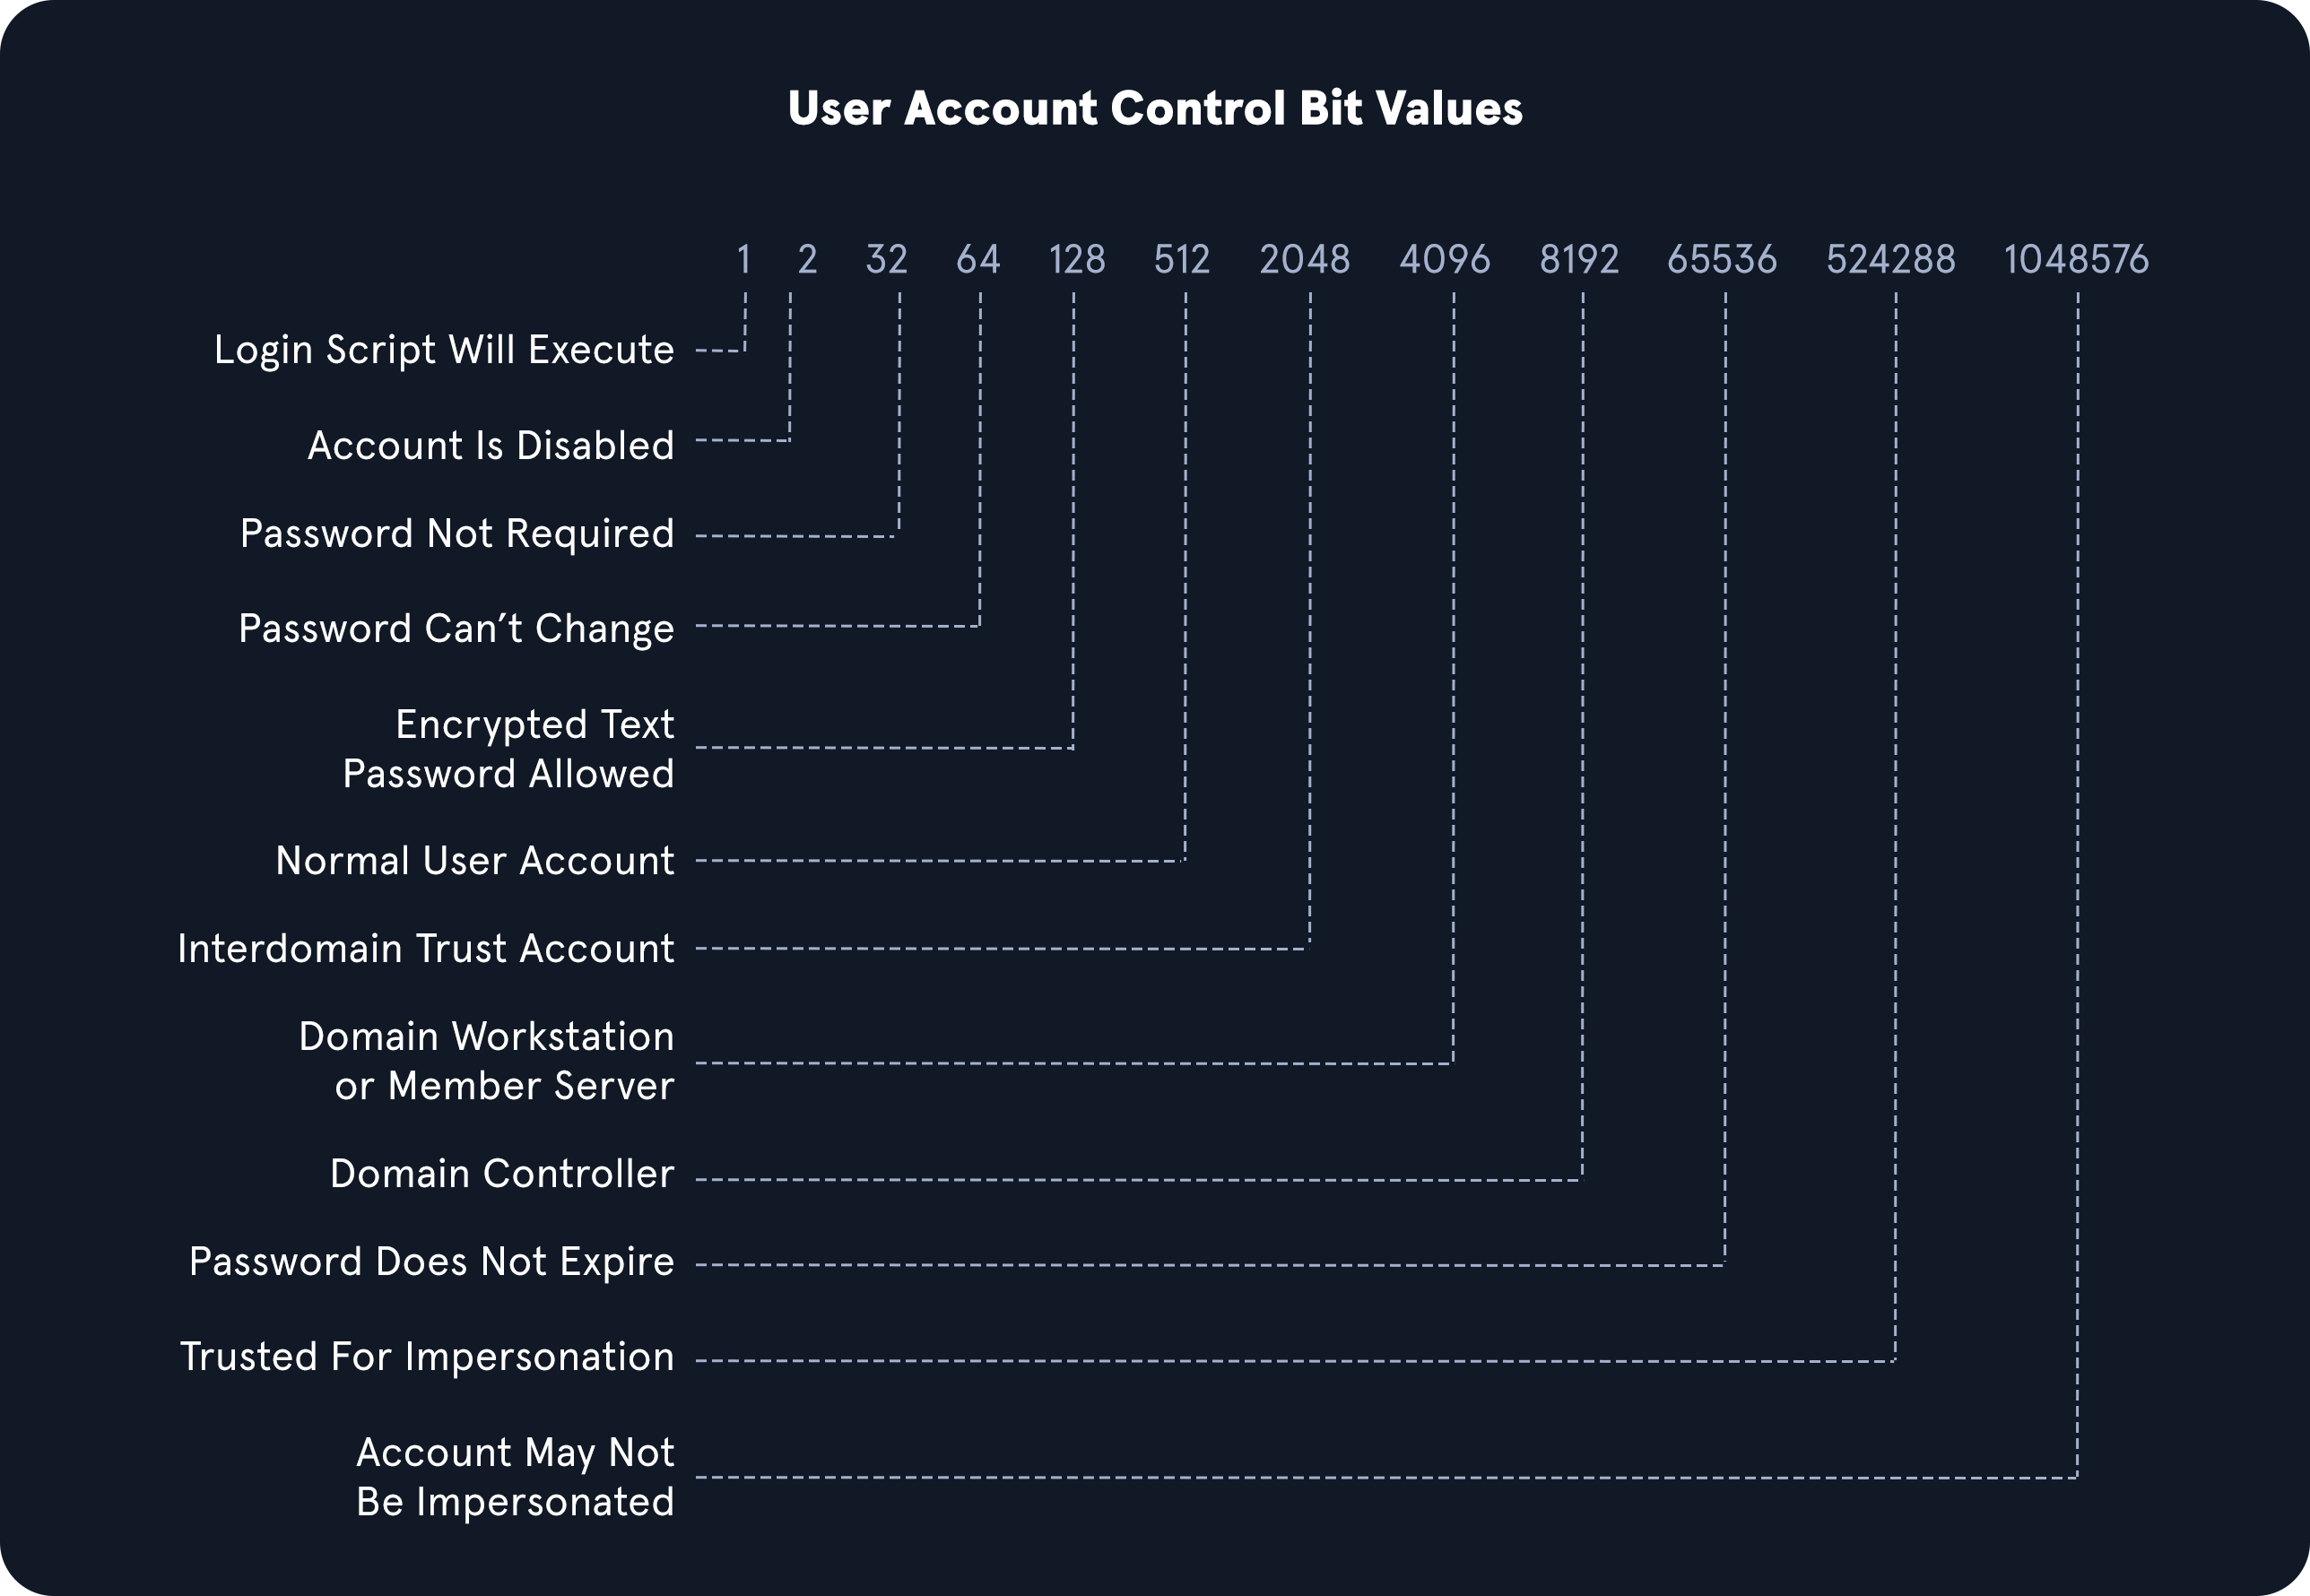
\includegraphics[width=\linewidth]{ad/knowledge/images/UAC-values.png}
  \caption{Some Important UAC flag attribute values}
  \label{fig:uac-values}
\end{figure}

\subsubsection{links}

\begin{itemize}
    \item \url{https://docs.microsoft.com/en-us/windows/security/identity-protection/user-account-control/user-account-control-overview}

    \item \url{https://docs.microsoft.com/en-us/windows/security/identity-protection/user-account-control/how-user-account-control-works}
    \item
        \url{https://docs.microsoft.com/en-us/troubleshoot/windows-server/identity/useraccountcontrol-manipulate-account-properties}
\end{itemize}


